\section{Memory Characteristics}
We now discuss the memory behavior of pipelining and non-pipelining strategies.
We first formulate the memory footprint of these two strategies individually, and then compare their memory behavior with each other. 

\begin{figure}[t]
	\centering 
	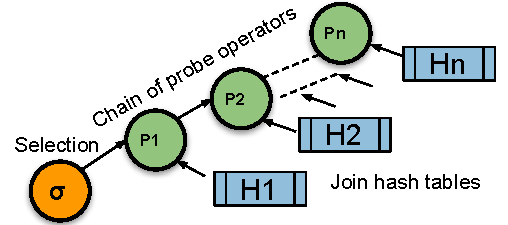
\includegraphics{figures/Left-deep-pipeline}
	\caption{\textbf{A left-deep query plan fragment that shows a pipeline of selection and multiple probe operators}}
	\label{fig:left-deep-plan}
\end{figure}

Let us consider a pipeline of selection and multiple probe operators as shown in Figure~\ref{fig:left-deep-plan}.
We are interested in finding out the \textit{active memory} used by pipelining and non-pipelining strategy.
Before we present the analysis, here are our assumptions:
As soon as a probe operation on an input block is over, the input block can be safely removed from the buffer pool.
We can make this assumption, because the materialization after probe operation preserves the necessary attributes from the input and hence the original input block is not necessary.
We assume that memory allocation happens in chunks, and each chunk has the same size. 
This assumption is realistic as many systems use system calls like \texttt{mmap()} or \texttt{malloc()} for allocating memory.

We assume a left-deep pipeline that starts at a selection operator and has multiple probe operators.
\todo{complete the section}